\subsection{Faster R-CNN}
\begin{frame}{}
    \LARGE Object Detection: \textbf{Faster R-CNN}
\end{frame}

\begin{frame}{Faster R-CNN}
    \begin{itemize}
        \item Make CNN do proposals!
        \item Insert Region Proposal Network (RPN) to predict proposals from features
        \pause
        \item Jointly train on 4 losses:
        \begin{itemize}
            \item \textbf{RPN classification:} anchor box is object / not an object
            \item \textbf{RPN regression:} predict transform from anchor box to proposal box
            \item \textbf{Object classification:} classify proposals as background / object class
            \item \textbf{Object regression:} predict transform from proposal box to object box
        \end{itemize}
    \end{itemize}
    
\end{frame}

\begin{frame}[allowframebreaks]{Faster R-CNN}
    \begin{figure}
        \centering
        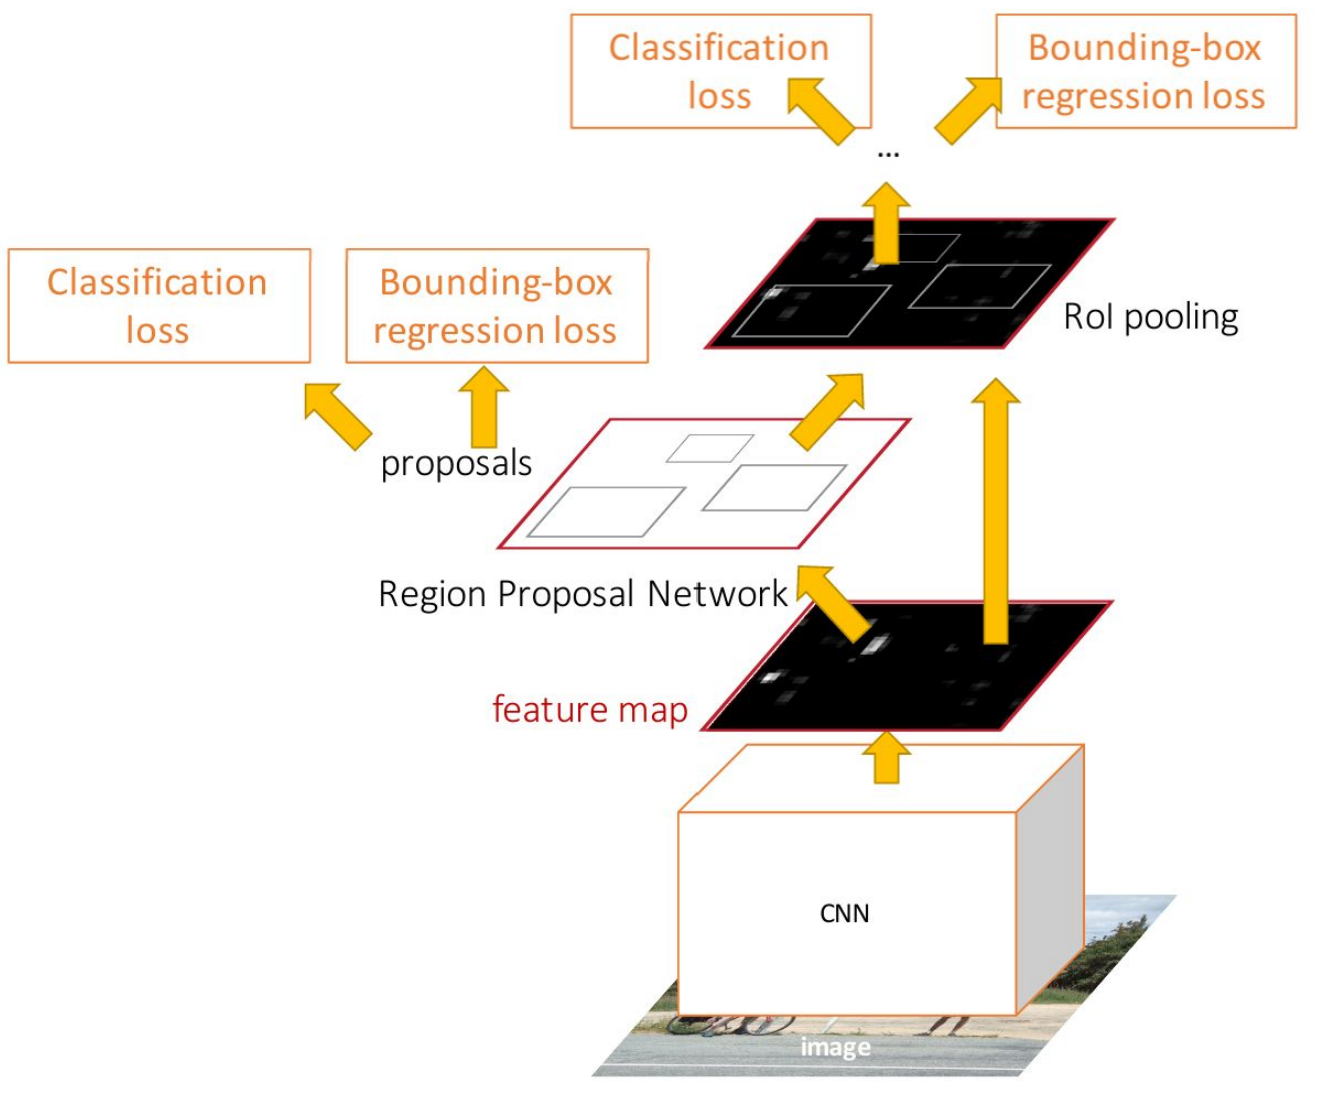
\includegraphics[width=1.0\textwidth,height=0.9\textheight,keepaspectratio]{images/object-detect/faster_rcnn_1.png}
    \end{figure}

\framebreak

    \begin{figure}
        \centering
        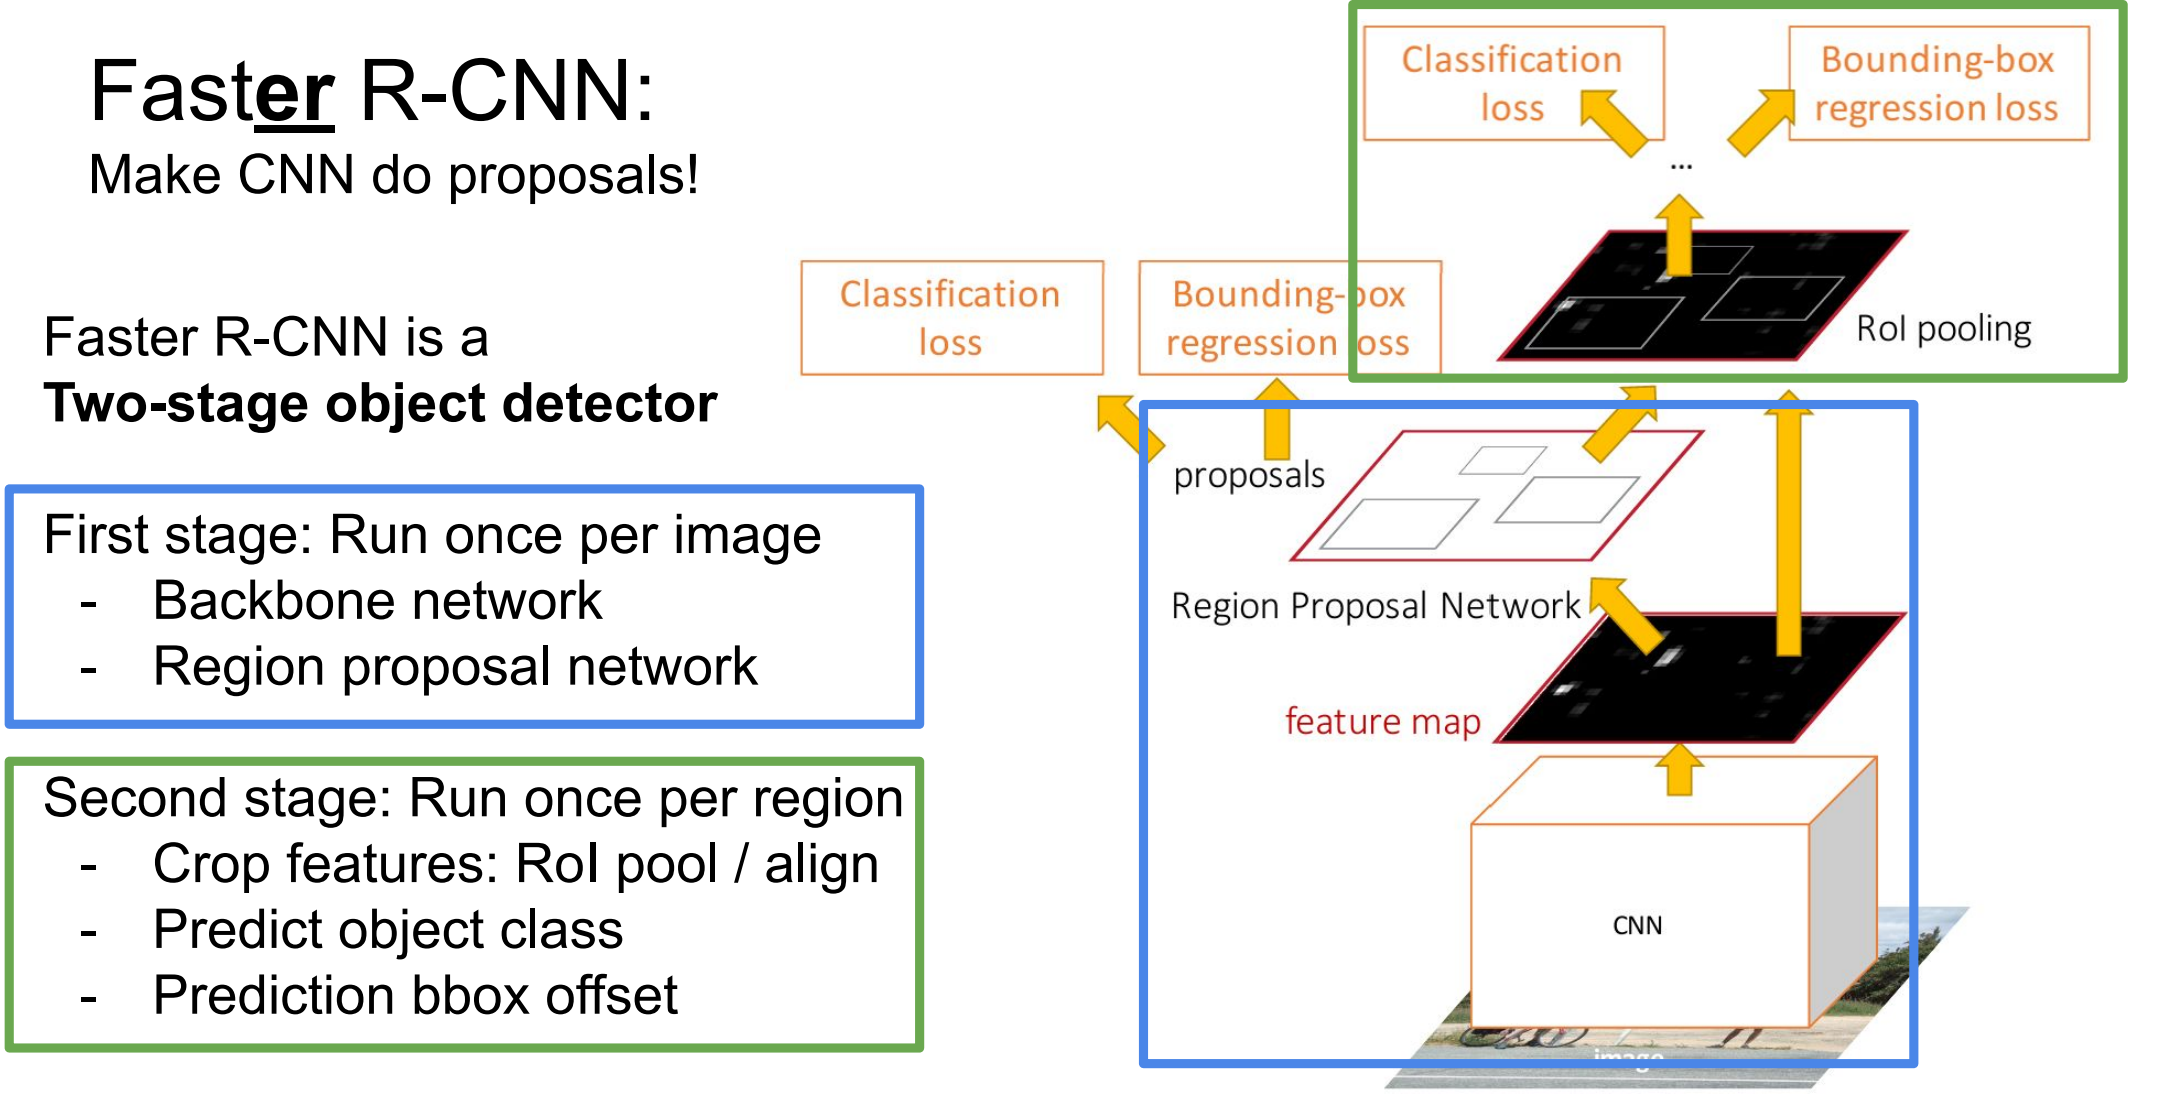
\includegraphics[width=1.0\textwidth,height=1.0\textheight,keepaspectratio]{images/object-detect/faster_rcnn_2.png}
    \end{figure}

\framebreak

    \begin{figure}
        \centering
        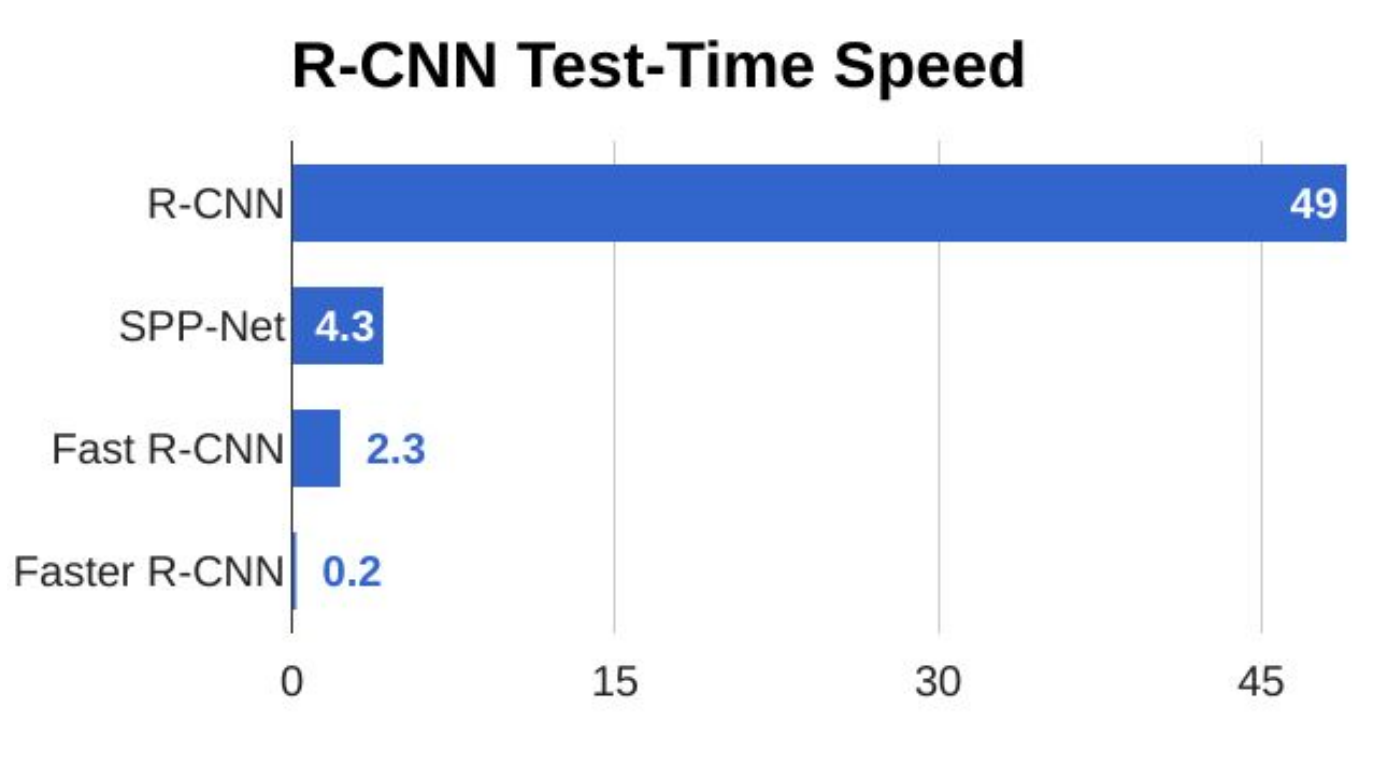
\includegraphics[width=1.0\textwidth,height=1.0\textheight,keepaspectratio]{images/object-detect/faster_rcnn_3.png}
    \end{figure}
\end{frame}